\section{R has a built-in dataset called {\color{red} trees} that contains observations for 
    $n = 31$ black cherry
    trees. The first column, “Girth,” contains the girth of the trees (in inches); the second
    column, “Height,” contains the height of the trees (in feet); the third column, “Volume,”
    contains the volume of timber (in cubic feet).}
    \begin{multicols}{2}
        \subsection{State the least-squares estimate of the model predicting diameter from height.}
            (Note: Diameter is mislabeled as girth in the dataset.)\\
            $d$ and $h$ are in inches: $d \approx 0.02131h-6.188$

        \subsection{Predict the diameters of trees of the following heights: 
            $60$ feet, $73$ feet, and $85$ feet.}
            In inches.\\
            Height of 60 feet: \\
            $d \approx 0.02131226 (60 * 12)-6.18839451$
            $\approx 9.156$\\
            Height of 73 feet: \\
            $d \approx 0.02131226 (73 * 12)-6.18839451$
            $\approx 12.48$\\
            Height of 85 feet: \\
            $d \approx 0.02131226 (85 * 12)-6.18839451$
            $\approx 15.55$

        \subsection{Interpret the meaning of the slope in the context of the data.}
            For every 1 inch increase the height, 
            there will be a 0.02131 inch increase in diameter.

        \subsection{Suppose you wanted to conduct a hypothesis test for a positive linear relationship
            between height and diameter. State the appropriate hypotheses and test statistic.}
            $H_0: \beta_1 \leq 0, H_a: \beta_1 > 0$\\
            $t = \frac{\beta_1 - \beta_{1_0}}{SE_{\beta_1}}
            \approx \frac{0.02131226 - 0}{ 0.006513191} \approx 3.272$

        \subsection{State the probability expression of the p-value as well as the p-value itself. What
            conclusion would we reach with respect to our hypotheses in part d. using $\alpha = 0.05$?}
            $\pv = P(T_{df} > 3.272\hdots) = 1 - pt(t, df) 
            \approx 0.1379\% < 5\% = \alpha$\\
            Therefore there is a linear dependency of height on diameter.

        \subsection{If you wanted to report a $95\%$ interval for the diameter of a single tree that was $80$
            feet tall, would you report a confidence interval or prediction interval? Why?}
            Prediction interval, as it predicts the dependent variable 
            from a given independent variable\\
            Prediction interval: (13.08276, 15.45999 ) in inches.

        \subsection{What proportion of $\sigma^2$ in diameter is explained by its linear relationship with
            height?}
            $r^2 \approx 0.2697$

        \subsection{Examine the residual plot. What condition/assumption does the residual plot check for?
            Does it appear to be met in this case?}
            %See figure \ref{fig:3h} on page \pageref{fig:3h}.
            It checks for consistancy in variance. 
            In this case, yes, the points are in a random pattern.
            \begin{center}
                % Created by tikzDevice version 0.12.3 on 2019-08-18 21:40:24
% !TEX encoding = UTF-8 Unicode
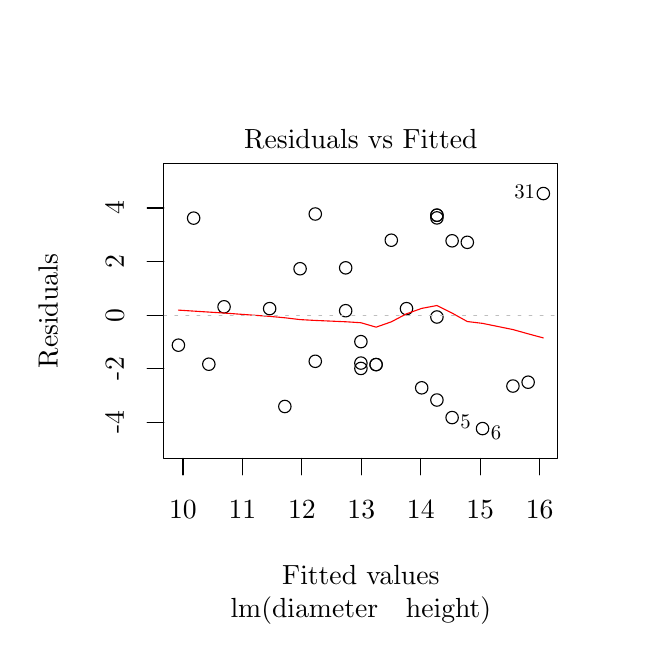
\begin{tikzpicture}[x=1pt,y=1pt]
\definecolor{fillColor}{RGB}{255,255,255}
\path[use as bounding box,fill=fillColor,fill opacity=0.00] (0,0) rectangle (216.81,216.81);
\begin{scope}
\path[clip] (  0.00,  0.00) rectangle (216.81,216.81);
\definecolor{drawColor}{RGB}{0,0,0}

\path[draw=drawColor,line width= 0.4pt,line join=round,line cap=round] ( 56.11, 61.20) -- (185.01, 61.20);

\path[draw=drawColor,line width= 0.4pt,line join=round,line cap=round] ( 56.11, 61.20) -- ( 56.11, 55.20);

\path[draw=drawColor,line width= 0.4pt,line join=round,line cap=round] ( 77.60, 61.20) -- ( 77.60, 55.20);

\path[draw=drawColor,line width= 0.4pt,line join=round,line cap=round] ( 99.08, 61.20) -- ( 99.08, 55.20);

\path[draw=drawColor,line width= 0.4pt,line join=round,line cap=round] (120.56, 61.20) -- (120.56, 55.20);

\path[draw=drawColor,line width= 0.4pt,line join=round,line cap=round] (142.05, 61.20) -- (142.05, 55.20);

\path[draw=drawColor,line width= 0.4pt,line join=round,line cap=round] (163.53, 61.20) -- (163.53, 55.20);

\path[draw=drawColor,line width= 0.4pt,line join=round,line cap=round] (185.01, 61.20) -- (185.01, 55.20);

\node[text=drawColor,anchor=base,inner sep=0pt, outer sep=0pt, scale=  1.00] at ( 56.11, 39.60) {10};

\node[text=drawColor,anchor=base,inner sep=0pt, outer sep=0pt, scale=  1.00] at ( 77.60, 39.60) {11};

\node[text=drawColor,anchor=base,inner sep=0pt, outer sep=0pt, scale=  1.00] at ( 99.08, 39.60) {12};

\node[text=drawColor,anchor=base,inner sep=0pt, outer sep=0pt, scale=  1.00] at (120.56, 39.60) {13};

\node[text=drawColor,anchor=base,inner sep=0pt, outer sep=0pt, scale=  1.00] at (142.05, 39.60) {14};

\node[text=drawColor,anchor=base,inner sep=0pt, outer sep=0pt, scale=  1.00] at (163.53, 39.60) {15};

\node[text=drawColor,anchor=base,inner sep=0pt, outer sep=0pt, scale=  1.00] at (185.01, 39.60) {16};

\path[draw=drawColor,line width= 0.4pt,line join=round,line cap=round] ( 49.20, 74.25) -- ( 49.20,151.66);

\path[draw=drawColor,line width= 0.4pt,line join=round,line cap=round] ( 49.20, 74.25) -- ( 43.20, 74.25);

\path[draw=drawColor,line width= 0.4pt,line join=round,line cap=round] ( 49.20, 93.60) -- ( 43.20, 93.60);

\path[draw=drawColor,line width= 0.4pt,line join=round,line cap=round] ( 49.20,112.95) -- ( 43.20,112.95);

\path[draw=drawColor,line width= 0.4pt,line join=round,line cap=round] ( 49.20,132.31) -- ( 43.20,132.31);

\path[draw=drawColor,line width= 0.4pt,line join=round,line cap=round] ( 49.20,151.66) -- ( 43.20,151.66);

\node[text=drawColor,rotate= 90.00,anchor=base,inner sep=0pt, outer sep=0pt, scale=  1.00] at ( 34.80, 74.25) {-4};

\node[text=drawColor,rotate= 90.00,anchor=base,inner sep=0pt, outer sep=0pt, scale=  1.00] at ( 34.80, 93.60) {-2};

\node[text=drawColor,rotate= 90.00,anchor=base,inner sep=0pt, outer sep=0pt, scale=  1.00] at ( 34.80,112.95) {0};

\node[text=drawColor,rotate= 90.00,anchor=base,inner sep=0pt, outer sep=0pt, scale=  1.00] at ( 34.80,132.31) {2};

\node[text=drawColor,rotate= 90.00,anchor=base,inner sep=0pt, outer sep=0pt, scale=  1.00] at ( 34.80,151.66) {4};

\path[draw=drawColor,line width= 0.4pt,line join=round,line cap=round] ( 49.20, 61.20) --
	(191.61, 61.20) --
	(191.61,167.61) --
	( 49.20,167.61) --
	( 49.20, 61.20);
\end{scope}
\begin{scope}
\path[clip] (  0.00,  0.00) rectangle (216.81,216.81);
\definecolor{drawColor}{RGB}{0,0,0}

\node[text=drawColor,anchor=base,inner sep=0pt, outer sep=0pt, scale=  1.00] at (120.41, 15.60) {Fitted values};

\node[text=drawColor,rotate= 90.00,anchor=base,inner sep=0pt, outer sep=0pt, scale=  1.00] at ( 10.80,114.41) {Residuals};
\end{scope}
\begin{scope}
\path[clip] ( 49.20, 61.20) rectangle (191.61,167.61);
\definecolor{drawColor}{RGB}{0,0,0}

\path[draw=drawColor,line width= 0.4pt,line join=round,line cap=round] ( 92.93, 79.92) circle (  2.25);

\path[draw=drawColor,line width= 0.4pt,line join=round,line cap=round] ( 65.46, 95.20) circle (  2.25);

\path[draw=drawColor,line width= 0.4pt,line join=round,line cap=round] ( 54.47,102.08) circle (  2.25);

\path[draw=drawColor,line width= 0.4pt,line join=round,line cap=round] (103.92, 96.26) circle (  2.25);

\path[draw=drawColor,line width= 0.4pt,line join=round,line cap=round] (153.37, 75.92) circle (  2.25);

\path[draw=drawColor,line width= 0.4pt,line join=round,line cap=round] (164.36, 71.94) circle (  2.25);

\path[draw=drawColor,line width= 0.4pt,line join=round,line cap=round] ( 70.96,115.95) circle (  2.25);

\path[draw=drawColor,line width= 0.4pt,line join=round,line cap=round] (120.41, 93.67) circle (  2.25);

\path[draw=drawColor,line width= 0.4pt,line join=round,line cap=round] (147.88, 82.26) circle (  2.25);

\path[draw=drawColor,line width= 0.4pt,line join=round,line cap=round] (120.41, 95.61) circle (  2.25);

\path[draw=drawColor,line width= 0.4pt,line join=round,line cap=round] (142.38, 86.67) circle (  2.25);

\path[draw=drawColor,line width= 0.4pt,line join=round,line cap=round] (125.90, 95.07) circle (  2.25);

\path[draw=drawColor,line width= 0.4pt,line join=round,line cap=round] (125.90, 95.07) circle (  2.25);

\path[draw=drawColor,line width= 0.4pt,line join=round,line cap=round] ( 87.44,115.29) circle (  2.25);

\path[draw=drawColor,line width= 0.4pt,line join=round,line cap=round] (120.41,103.35) circle (  2.25);

\path[draw=drawColor,line width= 0.4pt,line join=round,line cap=round] (114.91,114.53) circle (  2.25);

\path[draw=drawColor,line width= 0.4pt,line join=round,line cap=round] (175.35, 87.31) circle (  2.25);

\path[draw=drawColor,line width= 0.4pt,line join=round,line cap=round] (180.84, 88.70) circle (  2.25);

\path[draw=drawColor,line width= 0.4pt,line join=round,line cap=round] ( 98.43,129.70) circle (  2.25);

\path[draw=drawColor,line width= 0.4pt,line join=round,line cap=round] ( 59.97,147.99) circle (  2.25);

\path[draw=drawColor,line width= 0.4pt,line join=round,line cap=round] (136.89,115.28) circle (  2.25);

\path[draw=drawColor,line width= 0.4pt,line join=round,line cap=round] (147.88,112.26) circle (  2.25);

\path[draw=drawColor,line width= 0.4pt,line join=round,line cap=round] (114.91,130.02) circle (  2.25);

\path[draw=drawColor,line width= 0.4pt,line join=round,line cap=round] (103.92,149.48) circle (  2.25);

\path[draw=drawColor,line width= 0.4pt,line join=round,line cap=round] (131.39,140.01) circle (  2.25);

\path[draw=drawColor,line width= 0.4pt,line join=round,line cap=round] (153.37,139.79) circle (  2.25);

\path[draw=drawColor,line width= 0.4pt,line join=round,line cap=round] (158.86,139.25) circle (  2.25);

\path[draw=drawColor,line width= 0.4pt,line join=round,line cap=round] (147.88,148.07) circle (  2.25);

\path[draw=drawColor,line width= 0.4pt,line join=round,line cap=round] (147.88,149.04) circle (  2.25);

\path[draw=drawColor,line width= 0.4pt,line join=round,line cap=round] (147.88,149.04) circle (  2.25);

\path[draw=drawColor,line width= 0.4pt,line join=round,line cap=round] (186.34,156.87) circle (  2.25);
\definecolor{drawColor}{RGB}{255,0,0}

\path[draw=drawColor,line width= 0.4pt,line join=round,line cap=round] ( 54.47,114.75) --
	( 59.97,114.39) --
	( 65.46,114.04) --
	( 70.96,113.69) --
	( 87.44,112.49) --
	( 92.93,111.98) --
	( 98.43,111.32) --
	(103.92,111.02) --
	(103.92,111.02) --
	(114.91,110.54) --
	(114.91,110.54) --
	(120.41,110.19) --
	(120.41,110.19) --
	(120.41,110.19) --
	(125.90,108.59) --
	(125.90,108.59) --
	(131.39,110.51) --
	(136.89,113.41) --
	(142.38,115.37) --
	(147.88,116.41) --
	(147.88,116.41) --
	(147.88,116.41) --
	(147.88,116.41) --
	(147.88,116.41) --
	(153.37,113.67) --
	(153.37,113.67) --
	(158.86,110.62) --
	(164.36,109.96) --
	(175.35,107.72) --
	(180.84,106.18) --
	(186.34,104.70);
\end{scope}
\begin{scope}
\path[clip] (  0.00,  0.00) rectangle (216.81,216.81);
\definecolor{drawColor}{RGB}{0,0,0}

\node[text=drawColor,anchor=base,inner sep=0pt, outer sep=0pt, scale=  1.00] at (120.41,  3.60) {lm(diameter ~ height)};
\end{scope}
\begin{scope}
\path[clip] (  0.00,  0.00) rectangle (216.81,216.81);
\definecolor{drawColor}{RGB}{0,0,0}

\node[text=drawColor,anchor=base,inner sep=0pt, outer sep=0pt, scale=  1.00] at (120.41,173.01) {Residuals vs Fitted};
\end{scope}
\begin{scope}
\path[clip] (  0.00,  0.00) rectangle (216.81,216.81);
\definecolor{drawColor}{RGB}{0,0,0}

\node[text=drawColor,anchor=base east,inner sep=0pt, outer sep=0pt, scale=  0.75] at (183.34,155.15) {31};

\node[text=drawColor,anchor=base west,inner sep=0pt, outer sep=0pt, scale=  0.75] at (167.36, 67.92) {6};

\node[text=drawColor,anchor=base west,inner sep=0pt, outer sep=0pt, scale=  0.75] at (156.37, 71.90) {5};
\end{scope}
\begin{scope}
\path[clip] ( 49.20, 61.20) rectangle (191.61,167.61);
\definecolor{drawColor}{RGB}{190,190,190}

\path[draw=drawColor,line width= 0.4pt,dash pattern=on 1pt off 3pt ,line join=round,line cap=round] ( 49.20,112.95) -- (191.61,112.95);
\end{scope}
\end{tikzpicture}

            \end{center}
    \end{multicols}